\chapter{Schéma entités-associations}

\begin{figure}
  \centering
  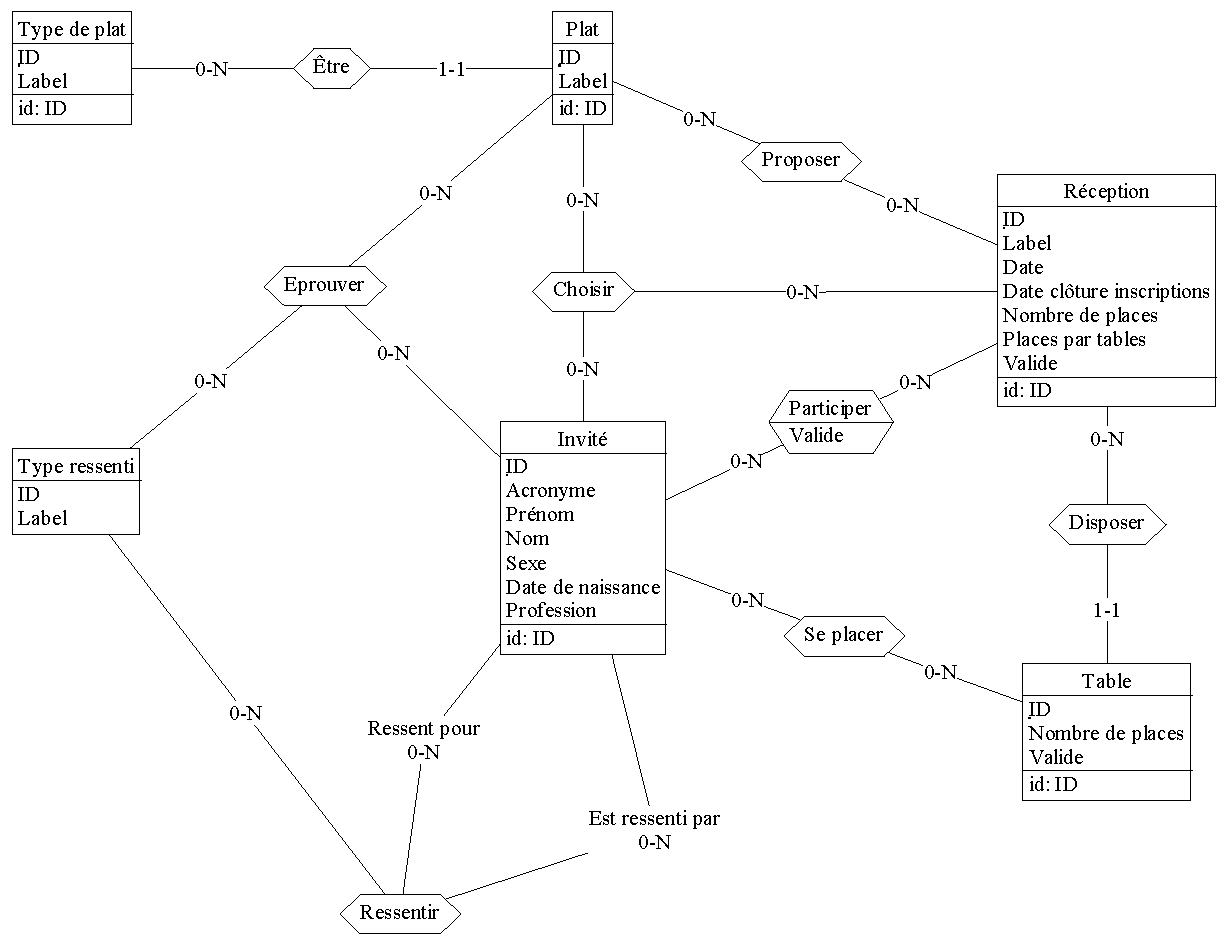
\includegraphics[width=\textwidth]{IMG/ea}
  \caption{Schéma entités-associations}
  \label{img_ea}
\end{figure}

La figure \refpage{img_ea} représente notre schéma entités-associations. Associé aux règles métier définies au chapitre \refpage{chapter_business_rules}, il permettra d'implémenter notre base de données et d'y définir nos contraintes.

Ce modèle est volontairement simpliste. Il sera nécessaire de définir des vues afin de présenter au mieux les données, comme par exemple les menus ou le plan de table.